\documentclass[../../main.tex]{subfiles}
\begin{document}

\section{Medici\'on corriente de bias y tensi\'on de offset}


\begin{circuitikz}
  		\draw (0,0) node[op amp][yscale=-1] (opamp) {}
  		(opamp.-) 	to[short]($(opamp.-)-(0.5,0)$) 
  					to[short]($(opamp.-)-(0.5, 1.5)$)
  					to[R=$R_1$]($(opamp.-)-(0.5,3)$)
  					node [ground]{}
  		($(opamp.-)-(0.5, 1.5)$) to[R=$R_2$] ($(opamp.-)-(-2.38, 1.5)$)
  					to[short]($(opamp.out)$)
  					
  		(opamp.+) to[short] ($(opamp.+)-(2,0)$)
  				  to[R=$R_3$]($(opamp.+)-(3.5,0)$)
  				  to[sV=$V_{in}$]($(opamp.-)-(3.5,3)$) node[ground]{}
  				  

		($(opamp.+)-(1.5,0)$) to[R=$R_4$] ($(opamp.-)-(1.5,3)$) node[ground] {}
		
		(opamp.out) to ($(opamp.out)+(1,0)$) node[ocirc]{$\,\, V_{out}$}
  		
  		;
\end{circuitikz}



\subsection{Modelo de amplificador operacional con corrientes de bias y tensi\'on de offset}

\begin{figure}[htb]	%modelo opamp vio ibias
	\centering
	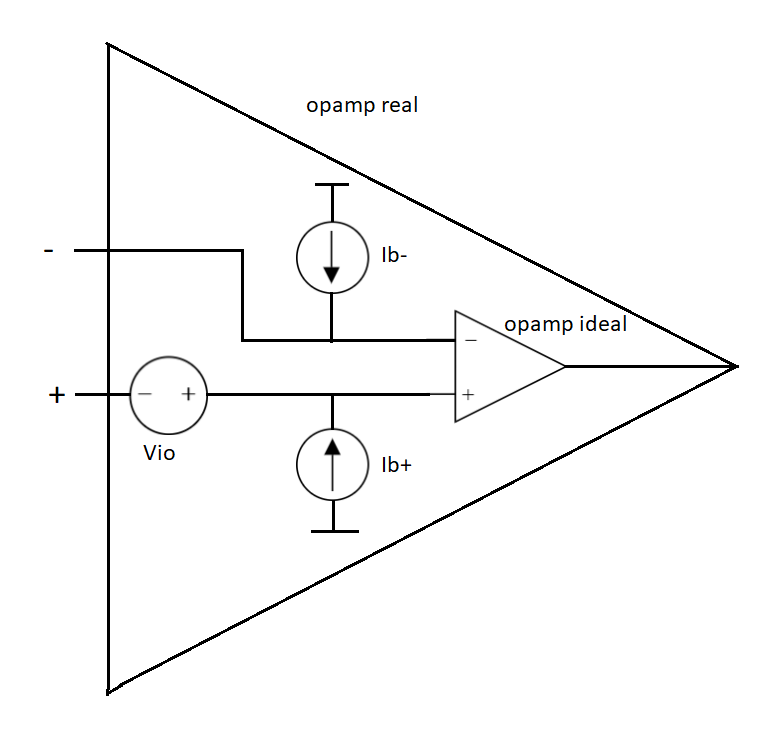
\includegraphics[width=0.4\textwidth]{imagenes/modelo_opamp_vio_ibias.png}
	\caption{Modelo de amplificador operacional con corrientes de bias y tensi\'on de offset}
	\label{fig:ej_3_modelo_opamp_vio_ibias}
\end{figure}

\todo[inline]{Que es corriente de bias y tension de offset. fijarme que puso roch en la intro}











\subsection{Importancia de las corrientes de bias y la tensi\'on de offset}


Las corrientes de bias($I_B^+$ y $I_B^-$) y la tensi\'on de offset ($V_{IO}$) pueden generar efectos que no concuerdan con el modelo ideal de un amplificador operacional. Se presentan a continuaci\'on tres ejemplos:

\subsubsection*{Efecto de $V_{IO}$}

\begin{figure}[htb]	%vio no despreciable
	\centering
	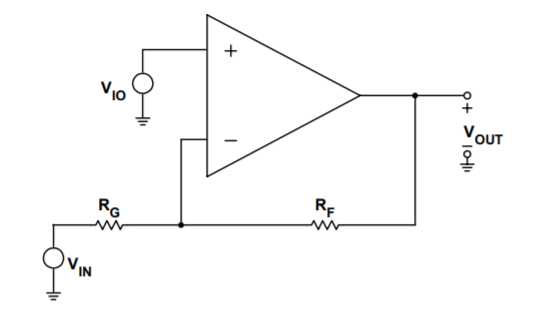
\includegraphics[height=0.2\textheight]{imagenes/vio_amplificacion.png}
	\caption{Modelo de amplificador con configuraci\'on inversora con $V_{IO}$ no despreciable}
	\label{fig:ej_3_efecto_vio}
\end{figure}

El circuito de la figura \ref{fig:ej_3_efecto_vio} representa un amplificador operacional en configuraci\'on inversora con tensi\'on de offset no despreciable modelado por un \textit{op-amp} ideal y una fuente de tensi\'on continua $V_{IO}$. De ignorarse la tensi\'on de offset, puede obtenerse la funci\'on transferencia:

\[\frac{V_{OUT}}{V_{IN}}=\frac{-R_F}{R_G}\]

Sin embargo, si se considera la tensi\'on de offset, no es posible obtener obtener la funci\'on transferencia ya que el sistema no es lineal:

\[V_{OUT}=V_{IN}\frac{-R_F}{R_G} + V_{IO}\left(1+\frac{R_F}{R_G}\right)\]
\[\text{Si }V_{IN} = 0,V_{OUT} = V_{IO}\left(1+\frac{R_F}{R_G}\right) \neq 0 \]
\[\Rightarrow \text{El sistema no es lineal}\]

Dependiendo el orden de $V_{IN}$ y de $V_{IO}$ y de la precisi\'on necesaria, el efecto de $V_{IO}$ en $V_{OUT}$ no puede ser despreciado.

\subsubsection*{Efecto de $I_B^+$ y $I_B^-$}
El amplificador operacional no puede funcionar si se impide el paso de las corrientes de bias. \todo{"impide el paso" suena medio choto pero no s\'e como decirlo m\'as mejor}Si se decide poner un capacitor en serie con una de las entradas, $I_B$ no podr\'a circular, haciendo que el amplificador no funcione correctamente. Ver ejemplo en figura \ref{fig:ej_3_GIC}. \todo{redaccion}

\begin{figure}[htb] %GIC
	\centering
	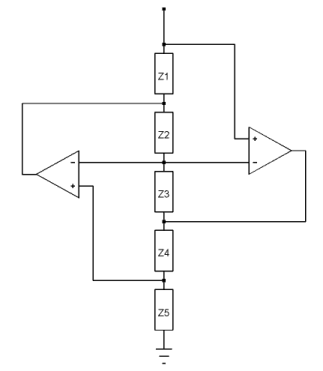
\includegraphics[width=0.35\textwidth]{imagenes/gic.png}
	\caption[Capacitores en un GIC]{Circuito GIC. Si $Z_2$ y $Z_3$ fueran capacitores, no podri\'ian circular las corrientes de bias. Una posible soluci\'on consiste en poner una resistencia en paralelo que permita la circulaci\'on y que sea lo suficientemente grande como para que la impedancia resultante sea aproximadamente capacituva pura.}
	\label{fig:ej_3_GIC}
\end{figure}


Por otro lado, si hay una resistencia $R$ en serie con la entrada del operacional, habr\'a una ca\'ida de tensi\'on $V=I_B^\pm\cdot R$ que puede o no ser despreciable dependiendo de la relaci\'on entre $I_B^\pm$ y $R$ y las caracter\'isticas del circuito. Este efecto es usado en el circuito de medici\'on explicado en la siguiente secci\'on para medir $I_B^+$ y $I_B^-$








\subsection{Circuitos con realimentaci\'on}	\label{ssec:realimentacion}

Un circuito realimentado es aquel en el que una proporcion de la salida se redirige a la entrada con el prop\'osito de controlar el comportamiento del sistema. Se  muestra un diagrama de un sistema realimentado t\'ipico en la figura \ref{fig:ej_3_realimentacion}
\footnote{Es com\'un encontrar el mismo modelo con la diferencia que a la entrada se le resta una se\~nal en vez de sumarse. Ambos modelos pueden representar los mismos sistemas (alcanza con cambiar la fase de $\beta$ en 180$^\circ$ para pasar de uno a otro). En este caso se decidi\'o usar la opici\'on con suma ya que es m\'as simple encontrar la similitud con el circuito analizado (ver siagrama de flujo de sen\~nal en la figura \ref{fig:ej_3_signal_flow_consigna_simplificado}}

\begin{description}
	\item[$A_{OL}$:] ganancia a lazo abierto del sistema (\textit{open-loop})
	\item[$A_{CL}$:] ganancia a lazo cerrado del sistema (\textit{closed-loop})
	\item[$A_{CL\,ideal}$:] ganancia a lazo cerrado ideal del sistema. $lim_{T\rightarrow \infty}A_{CL} = A_{CL\,ideal}$
	\item[$\beta$:] ganancia de realimentaci\'on
	\item[$T=A_{OL}\cdot\beta$:] ganancia de lazo
\end{description}

\begin{figure}[htbp] %diagrama realimentacion
	\centering
	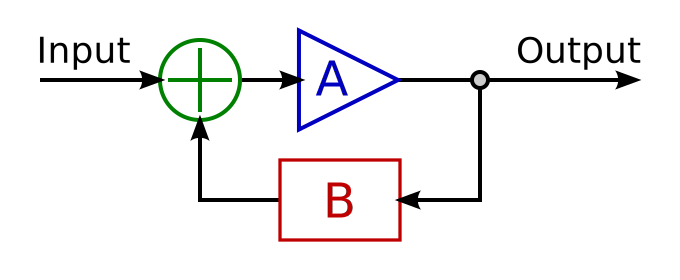
\includegraphics[width=0.5\textwidth]{imagenes/Ideal_feedback_model.png}
	\caption{Diagrama de flujo de se\~nal de sistemas realimentados.}
	\label{fig:ej_3_realimentacion}
\end{figure}


La funci\'on transferencia del sistema H(s) equivale a su ganancia a lazo cerrado:

\[x_d = x_i+x_f\]
\[x_f = \beta x_f\]
\[x_o = A_{OL}x_d = A_{OL}\left( x_i+x_f \right) =  A_{OL}\left( x_i+\beta x_o \right)\]
\[x_o - A_{OL} \beta x_o = A_{OL} x_i\]
\begin{equation}
	\Rightarrow H(s) = A_{CL} = \frac{x_o}{x_i} = \frac{A_{OL}}{1-A_{OL}\beta}
	\label{eq:ej_3_ACL}
\end{equation}

Suponiendo que $T\gg 1$ se obtiene la ganancia a lazo cerrado ideal:
\begin{equation}
	A_{CL\,ideal} = \frac{-1}{\beta}
	\label{eq:ej_3_ACL_IDEAL}
\end{equation}

Un sistema tiene realimentaci\'on negativa si la fase de la ganancia de lazo est\'a entre $180^\circ$ (inclusive) y $360^\circ$ (no inclusive)\todo{googlear algo de esto por que solo lo s\'e porque es palabra santo del senior, no tengo ninguna fuente}, y realimentaci\'on positiva en caso contrario.

\begin{figure}[htbp] %Ejemplo realimentacion negativa y positiva opamp
	\centering
	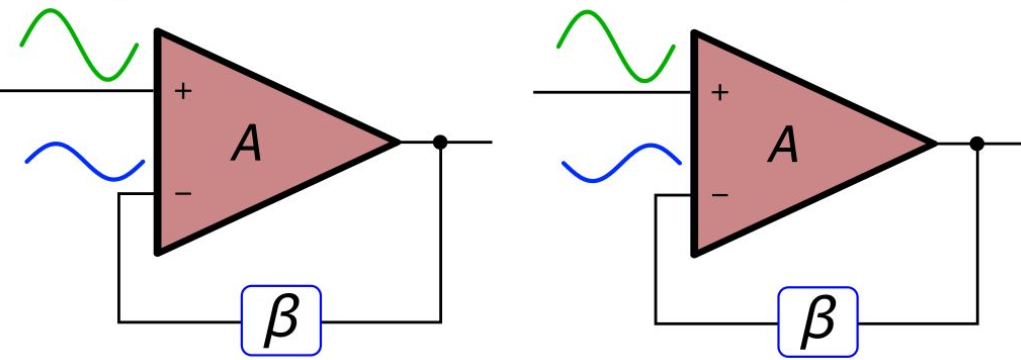
\includegraphics[width=0.5\textwidth]{imagenes/pos_vs_neg_feedback.png}
	\caption{Ejemplo de realimentaci\'on negativa y positiva en un \textit{op-amp}.}
	\label{fig:ej_3_realimentacion_pos_vs_neg_opamp}
\end{figure}










\subsection{Funcionamiento del circuito}
La funci\'on del circuito es medir la tensi\'on de offset y las corrientes de bias. La corriente de bias se obtiene midiendo la ca\'ida de tensi\'on que genera sobre una resistencia de $1M\Omega$. En la tabla \ref{tab:ej_3_datasheet} se observan los valores que se esperan medir.


\begin{table}[htbp]
\centering
\begin{tabular}{ccccccc}
               & \multicolumn{3}{c}{TL081}            & \multicolumn{3}{c}{LF356}    \\
\hline              
               & $V_{IO}$(mV) & $I_B$(pA) & $I_O$(pA) & $V_{IO}$(mV) & $I_B$(pA) & $I_O$(pA) \\
\hline
Valor t\'ipico & 3            & 30        & 5         & 3            & 30    & 3     \\
Valor m\'aximo & 6            & 200       & 100       & 10           & 200   & 50   
\end{tabular}
\end{table}

Todas las tensiones a determinar son amplificadas para as\'i aumentar la precisi\'on en la medici\'on. Una posibilidad ser\'ia amplificar a lazo abierto. Este m\'etodo cuenta con dos desventajas:
\begin{itemize}	%desventajas lazo abierto
	\item La ganancia a lazo abierto $A_{vol}$ t\'ipica de ambos amplificadores es 200V/mV. Con los valores de la tabla \ref{tab:ej_3_datasheet}, el amplificador saturar\'ia.
	\item Incluso si no hubiera saturaci\'on, \todo{redaccion: avol es super impreciso/ cambia una bocha entonces el resultado seria muy impreciso}
\end{itemize}
Por estos motivos se utiliza amplificaci\'on a lazo cerrado. En la figura \ref{fig:ej_3_medicion_vio_simple} se muestra un circuito de medici\'on de $V_{IO}$ con ganancia lazo cerrado. Sabiendo que la ganancia de un circuito de amplificacion no inversor es $1+\frac{R_2}{R_1}$, se obtiene $V_{IO}=\frac{R_1}{R_1+R_2}\cdot V_{OUT}$. 


\begin{figure}[htbp]	%medicion vio simplificado
	\centering
	\begin{subfigure}[t]{0.43\textwidth}
		\centering
		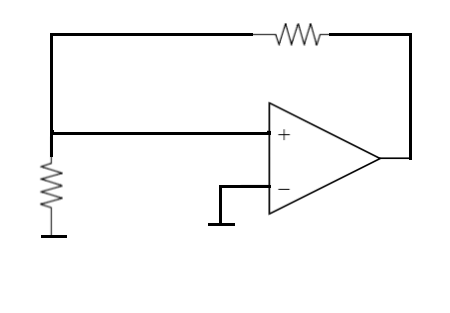
\includegraphics[width=\textwidth]{imagenes/medicion_vio_configuracion_simplificada.png}
		\caption{Con \textit{op-amp} real}
	\end{subfigure}%
	\hfill%%
	\begin{subfigure}[t]{0.43\textwidth}
		\centering
		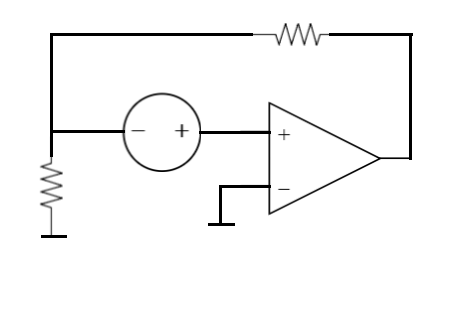
\includegraphics[width=\textwidth]{imagenes/medicion_vio_configuracion_simplificada_opamp_ideal.png}
		\caption{Con \textit{op-amp} ideal y fuente de tensi\'on modelando el \textit{op-amp} real y su tensi\'on de offset}
	\end{subfigure}	
	\caption[Circuito de medici\'on de $V_{IO}$ simplificado.]{Circuito de medici\'on de $V_{IO}$ simplificado.  $V_{OUT} = V_{IO} \cdot \left( 1+ \frac{R_2}{R_1} \right) $. No mide corrientes de bias y amplifica todas las frecuencias por igual.}
	\label{fig:ej_3_medicion_vio_simple}
\end{figure}

Ya que las se\~nales que se quieren medir tienen una amplitud comparable con el ruido que pueda llegar a inducirse en el circuito, es conveniente reducir la amplificaci\'on para las frecuencias mayores a cero. \todo{redaccion} Esto se logra en el circuito presentado en la consigna (figura \ref{fig:ej_3_medicion_vio_consigna})

\begin{figure}[htbp] %medicion vio ib+ ib- posta
	\centering
	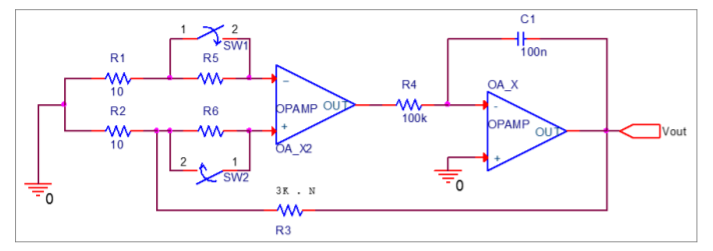
\includegraphics[scale=1]{imagenes/medicion_bias_configuracion_consigna.png}
	\caption{Circuito de medici\'on de $V_{IO}$, $I_B^+$ y $I_B^-$. El dispositivo cuyas caracter\'isticas se miden es el DUT, o \textit{device under test}, el cual es un amplificador con $V_{IO}$ y $I_B$ no despreciables.}
	\label{fig:ej_3_medicion_vio_consigna}
\end{figure}
\todo{grafico de consigna con los valores posta}
\begin{figure}[htbp] %medicion vio ib+ ib- posta con opamp ideal
	\centering
	\missingfigure[figwidth=\textwidth]{circuito con las fuentes}
	\caption{Mismo circuito que en la figura \ref{fig:ej_3_medicion_vio_consigna} cambiando el DUT por el modelo de la figura \ref{fig:ej_3_modelo_opamp_vio_ibias}}
	\label{fig:ej_3_medicion_vio_consigna_modelando}
\end{figure}

Se utiliza un diagrama de flujo de se\~nal (figura \ref{fig:ej_3_signal_flow_consigna_simplificado}) para obtener la funci\'on de transferencia del sistema. Se tomaron la siguiente consideraciones:
\begin{itemize}
	\item $\Delta V_{R1} = I_b^- \cdot 10\Omega \approx 0$
	\item $I_{R2}\approx I_{R3}$
	\item La ganancia a lazo abierto de ambos amplificadores es $A_{vol}$\footnote{Es importante distinguir la ganancia a lazo abierto de un \textit{op-amp} $A_{vol}$ de la ganancia a lazo abierto del circuito total $A_{OL}$ }
\end{itemize}


\begin{figure}[htpb]%signal flow consigna
	\centering
	\begin{subfigure}[t]{0.49\textwidth}
		\centering
		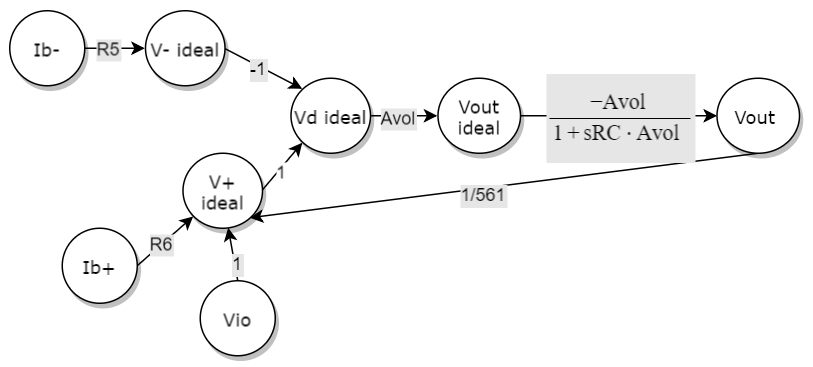
\includegraphics[width=\textwidth]{imagenes/signal_flow_consigna.png}
		\caption{Diagrama de flujo de se\~nal para el circuito de la consigna usando el modelo de la figura para el DUT}
		\label{fig:ej_3_signal_flow_consigna_no_simplificado}
	\end{subfigure}%
	\hfill%%
	\begin{subfigure}[t]{0.49\textwidth}
		\centering
		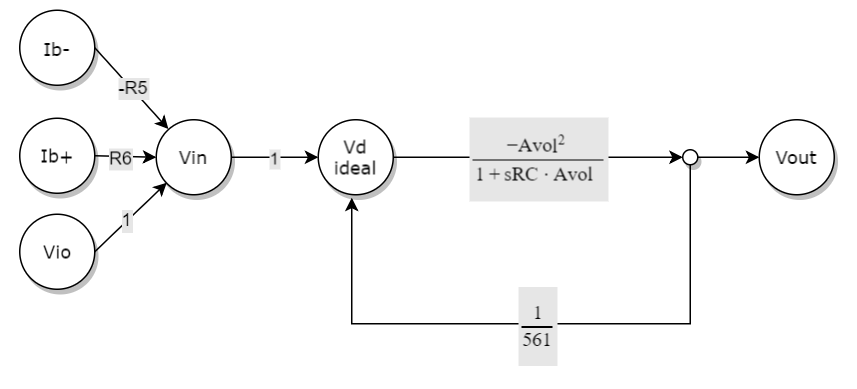
\includegraphics[width=\textwidth]{imagenes/signal_flow_consigna_simplificado.png}
		\caption{Simplificaci\'on del diagrama de flujo de se\~nal. La estructura coincide con la de un circuito con realimentacion (ver figura \ref{fig:ej_3_realimentacion}). }
		\label{fig:ej_3_signal_flow_consigna_simplificado}
	\end{subfigure}
	\label{fig:ej_3_signal_flow_consigna}	
\end{figure}


El diagrama de flujo de se\~nal coincide con el de un sistema realimentado descripto en la secci'on \ref{ssec:realimentacion}. La \'unica diferencia es que en este caso la entrada no es una \'unica se\~nal sino una suma:

\begin{equation}
	V_{in} = V_{IO} + I_B^+\cdot R6 - I_B^-\cdot R5
	\label{eq:ej_3_vin_aparente}
\end{equation}

Cabe destacar $V_{in}$ es una forma abstracta de agrupar los efectos generados por tres se\~nales reales distintas, y no corresponde necesariamente con una diferencia de potencial real entre dos puntos.

 Se puede obtener entonces la ganancia de lazo cerrado y la ganancia de realimentaci\'on del circuito:
\[\beta = \frac{1}{561}\]
\[A_{OL} = -\frac{A_{vol}^2}{1+sRC\cdot A_{vol}}\]

Con estos valores y teniendo en cuenta la ecuaci\'on \ref{eq:ej_3_ACL} se obtiene la funci\'on transferencia del sistema:

\begin{equation}
	H(s)=\frac{-\frac{A_{vol}^2}{1+sRC\cdot A_{vol}}}{1+\frac{A_{vol}}{1+sRC\cdot A_{vol}}\beta}
	=-\frac{1}{\frac{1}{A_{vol}^2}+\beta}\cdot \frac{1}{\frac{s}{\frac{1+A_{vol}^2\beta}{RCA_{vol}}} +1}
	\label{eg:ej_3_transferencia_consigna_sin_simplificar}
\end{equation}


Si se considera que $A_{vol}^2\beta \gg 1 \Rightarrow \beta \gg \frac{1}{A_{vol}^2}$ se puede simplificar la expresi\'on:


\begin{equation}
	H(s) = -\frac{1}{\beta}\cdot \frac{1}{\frac{s}{\frac{A_{vol}\beta}{RC}}+1}
	\label{eq:ej_3_transferencia_consigna_simplificada}
\end{equation}


Sabiendo que $lim_{T\rightarrow \infty}A_{CL} = A_{CL\,ideal}$:

\begin{equation}
	A_{CL\,ideal} = -\frac{1}{\beta} = -561
\end{equation}


\subsubsection{Funcionamiento en DC: mediciones de $V_{IO}$ y $I_B$}

Cuando $f=0$, evaluando en la funci\'on transferencia (ecuaci\'on \ref{eg:ej_3_transferencia_consigna_sin_simplificar}) se obtiene que la ganancia del circuito es $-\frac{1}{\beta}=-561$, por lo que $V_{in}=-\frac{V_{out}}{561}$


\begin{description}
	\item[Medici\'on de $V_{IO}$:] Cortocircuitando las resistencias R5 y R6 se obtiene que $V_{in} = V_{IO}$, valor que se puede obtener midiendo $V_{OUT}$:
	
	\[V_{IO} = -\frac{V_{OUT}}{561}\]
	\item[Medici\'on de $I_B^\pm$ y $I_B$:] Cortocircuitando R5 se obtiene $-\frac{V_{OUT}}{561} = V_{IO} + I_B^+\cdot R6$. Despejando:
	\[I_B^+=\frac{1}{R6}\cdot\left( -\frac{V_{OUT}}{561}-V_{IO}  \right) \]
	An\'alogamente,
	\[I_B^-=-\frac{1}{R5}\cdot \left( V_{IO} + \frac{V_{OUT}}{561}   \right)\]
	Una vez obtenidas $I_B^\pm$, se calcula $I_B$ definida como $\frac{I_B^++I_B^-}{2}$
\end{description}

\begin{table}[htbp]
\centering
\begin{tabular}{ccccc}
                       & \multicolumn{2}{c}{TL081} & \multicolumn{2}{c}{LF356} \\
\hline
Par\'ametro a calcular & $V_{OUT}$(mV)& Resultado  & $V_{OUT}$(mV)& Resultado  \\
\hline
$V_{IO}$               & 255          & -0,455mV   & 135          & -0,241mV   \\
$I_B^+$                & 0,675        & 453pA      & 0,179        & 241pA      \\
$I_B^-$                & 202          & -94,5pA    & 207          & -143pA     \\
$I_{IO}$			   &     ---      & 584 pA	   &	  ---     & 384pA      \\
$I_B$				   &     ---      & 179 pA     &      ---     & 49pA
\end{tabular}%

\caption{Resultados}
\label{tab:ej_3_resultados}
\end{table}

Las mediciones que son acordes a lo especificado en la hoja de datos son $V_{IO}$  y $I_B$ en los dos amplificadores. Por otro lado, se midieron valores de $I_O$ mayores al m\'aximo especificado por el fabricante, tambi\'en en los dos casos.



\subsubsection{Funcionamiento en AC}























\subsection{Estabilidad en diferentes configuraciones}




La estabilidad del sistema se analiza viendo la posici\'on de los polos en el plano complejo


En la figura \ref{fig:ej_3_realimentacion_pos_vs_neg_opamp} se muestran ejemplos de realimentaci\'on negativa y positiva en un amplificador operacional.



\subsubsection{Consigna}
\subsubsection{Uno invertido}
\subsubsection{Ambos invertidos}












\subsection{Medici\'on de $V_{IO}$ y $I_B^\pm$}


\begin{itemize}
	\item estabilidad
	\item inversion de los opamps
\end{itemize}

\end{document}
